\documentclass[]{article}
\usepackage[margin=0.9in]{geometry}

\usepackage{enumitem}
\usepackage{graphicx}
\usepackage{hyperref}
\usepackage{float}

\hypersetup{
	colorlinks=true,
	linkcolor=blue,
	filecolor=magenta,      
	urlcolor=cyan,
}

%opening
\title{User Manual for Docks}
\author{TripleParity}
\date{}

\begin{document}
	
\maketitle

\tableofcontents

\section{System Overview}
Docks is a system to manage a Docker Swarm using a Web User Interface. It provides a visual representation of a Docker Swarm, allowing users to manage the Swarm without using the Command Line Interface.

Docks is useful if you want to see a quick overview of the Swarm and all the running containers. Containers can be started and stopped with the click of a button.

System Administrators will be able to effectively manage their Swarm and scale services as required. Docks also appeals to users wishing to manage their services remotely from a web browser.

\section{System Configuration}
Docks consists of two subsystems; the Docks API server and the Docks UI.

The Docks API server has to be on a Manager Node in the Docker Swarm to be able to manage other nodes. The Docks UI also has to be served from the same Domain Name as the Docks API, in most cases it will also by deployed on the Manager Node.

\begin{figure}[h]
	\centering
	\includegraphics[scale=0.5]{pretty-docks.png}
\end{figure}

\pagebreak

\section{Installation}
\begin{enumerate}
	\item Install Docker (\url{https://docs.docker.com/install/})
	\item Install Docker Compose (\url{https://docs.docker.com/install/})
	\item Make sure the Docker Daemon is running (\url{https://docs.docker.com/config/daemon/})
	\item Clone the docks-demo repository using git (\url{https://github.com/TripleParity/docks-demo})
	\item Run \em{sudo docker-compose up -d} in the \em{docks-demo} folder that was cloned. This will start the Docks API on port `8080` and the web server on port `4200`. To view the output of the Dock API and web server, omit the `-d` flag. This process may take a while since Docker has to download the images for Docks
	\item Browse to \url{http://127.0.0.1:4200} to access the web interface.
	\item To stop the Docks UI and Docks API run \em{sudo docker-compose down} in the \em{docks-demo} folder to stop the running containers (docks and docks-ui)
\end{enumerate}


\section{Getting Started}
When using the docks-demo repository the UI will be available at \url{http://127.0.0.1:4200} after following the Installation instructions.

You will be presented with the following login screen:

\begin{figure}[H]
	\centering
	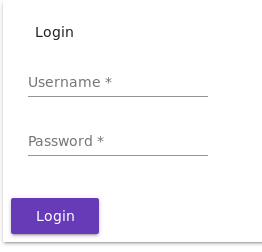
\includegraphics[scale=0.5]{manual_login.png}
	\caption{Docks Login Screen}
\end{figure}

Default credentials:
\begin{itemize}
	\item Username: "admin"
	\item password: "admin"
\end{itemize}

After logging in you will be presented with the Dashboard:
\begin{figure}[H]
	\centering
	
\includegraphics[scale=0.5]{manual_nav.png}
	\caption{Dashboard Navigation bar}
\end{figure}

\begin{figure}[H]
	\centering
	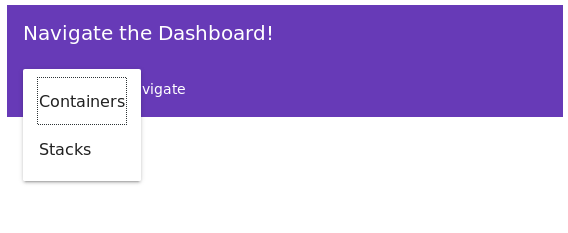
\includegraphics[scale=0.5]{manual_nav_select.png}
	\caption{Views}
\end{figure}

\begin{figure}[H]
	\centering
	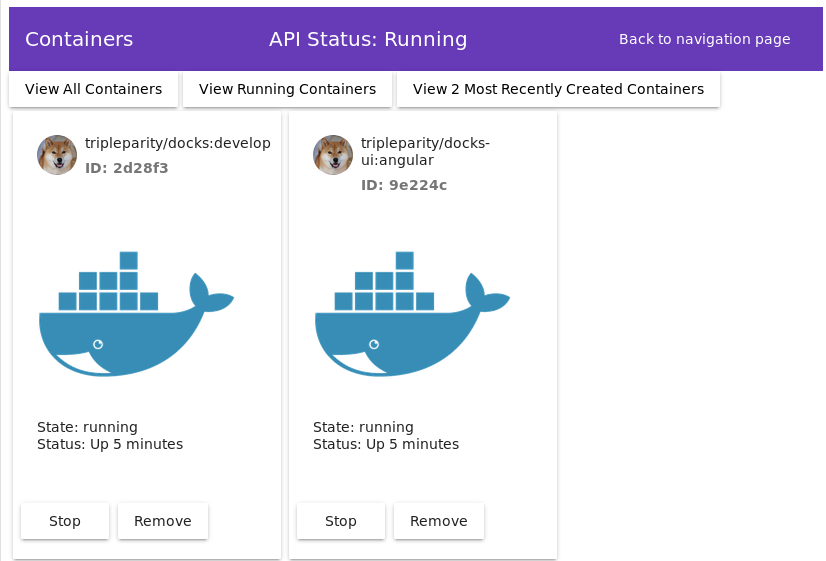
\includegraphics[scale=0.5]{manual_containers.png}
	\caption{Running containers}
\end{figure}

\section{Using the System}
\begin{itemize}
	\item Containers can be stopped by clicking the stop button. Simple.
	\item Containers can be removed by clicking the Remove button. Simple, again.
	\item More functionality will be added in future releases
\end{itemize}
\section{Troubleshooting}

\end{document}
